\addsec{Auswertung der Schülerumfrage}
\normalsize
Anzahl der Befragten: 147\\
Zeit der Befragung: 17. 11. 2020 - 01. 12. 2020\\\\\\
Wenn mehrere Antworten angegeben wurden, zählt jede je nach Frage entweder als eine Stimme(*) oder eine Stimme wird anteilmäßig auf die genannten Antwortmöglickeiten verteilt(**).\\\\\\\\\\\\\\\\
Würden Sie die folgenden Produkte eher Online oder vor Ort kaufen? (1)\\\\
\begin{figure}[H]
    \begin{center}
        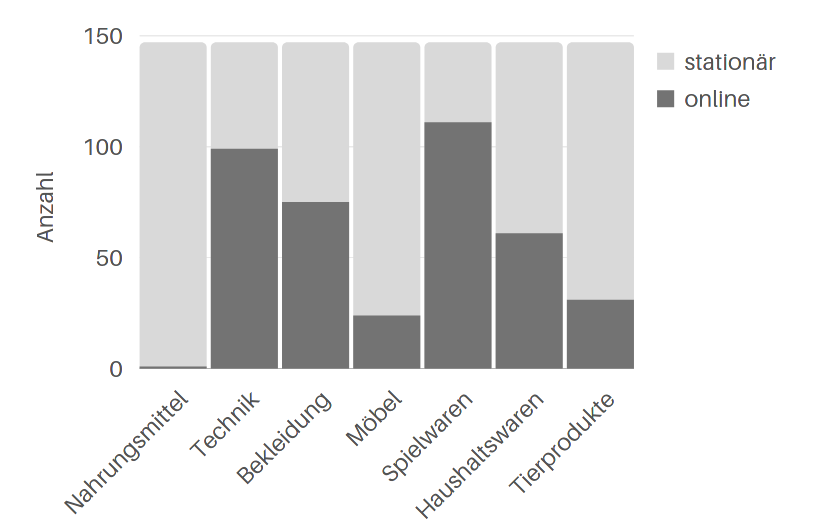
\includegraphics[width=12.5cm]{media/schuelerumfrage/1.png}
    \end{center}
\end{figure} 
\iffalse
Nahrungsmittel: 1 Online / 146 vor Ort

Technik: 99 Online / 47 vor Ort

Bekleidung: 74 Online / 72 vor Ort

Möbel: 24 Online / 122 vor Ort

Spielwaren: 111 Online / 36 vor Ort

Haushaltswaren: 61 Online / 86 vor Ort

Tierprodukte: 31 Online / 116 vor Ort\\\\
\fi 
\newpage\noindent Haben Sie schon einmal etwas Online bestellt, wenn ja über welche Plattform? (2)\\
\begin{figure}[H]
    \begin{center}
        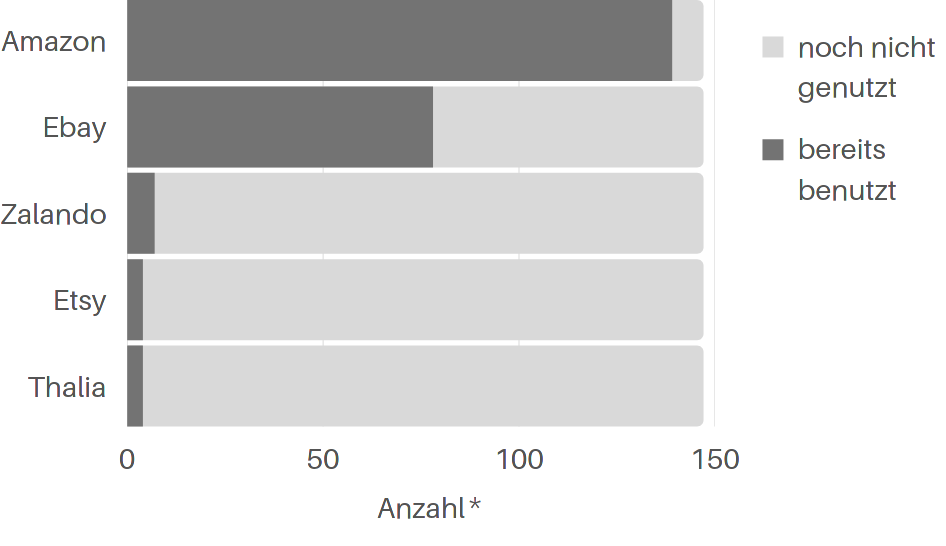
\includegraphics[width=11.5cm]{media/schuelerumfrage/2.png} 
    \end{center}
\end{figure}
\iffalse
Amazon: 139/147

Ebay: 78/147

Andere: Bershka(1), Shein(1), Zaful(3), Zalando(7), Etsy(4), H\&M(2), EMP(2), Maciag Offroad(1), Reifendirekt(1), Thalia(4), Böttcher AG(1), Globetrotter(1), Intersport(2)\\\\
\fi
\noindent Gibt es Artikel, die Sie nicht Online bestellen würden?** (3)\\
\begin{figure}[H]
    \begin{center}
        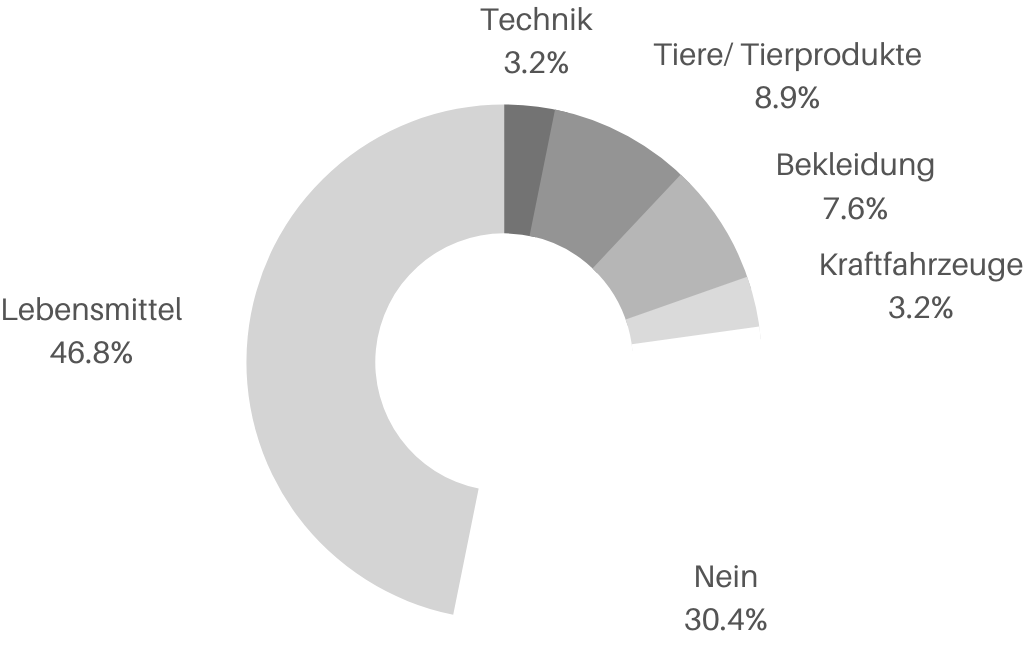
\includegraphics[width=11.5cm]{media/schuelerumfrage/3.png}
    \end{center}
\end{figure}
\iffalse
Nein: 48

Ja: Lebensmittel allgemein(23), Tiere(11), Nahrungsmittel(62), Tierwaren(7), Bekleidung(12), Technik(5), Kochbananen(1), Fahrzeuge(5), Mietwohnung(1), Gebrauchtwaren(3)\\\\
\fi

\newpage\noindent Wie beschreiben Sie ihre Erfahrungen mit dem Onlinehandel? (4)
\begin{figure}[H]
    \begin{center}
        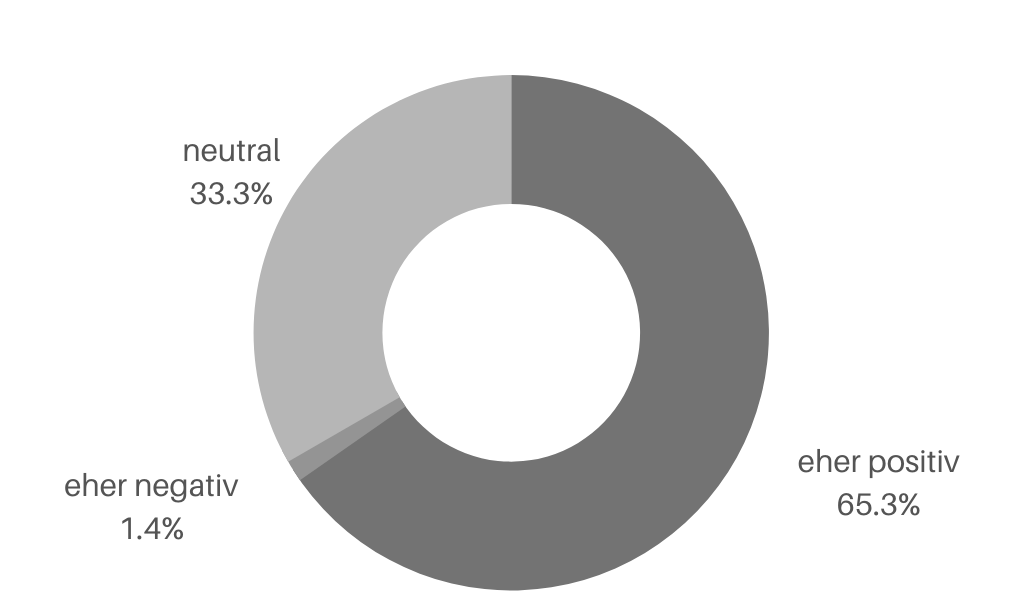
\includegraphics[width=11.5cm]{media/schuelerumfrage/4.png}
    \end{center}
\end{figure}
\iffalse
eher positiv: 96

eher negativ: 2

neutral: 49\\\\
\fi
\noindent Ist das Kaufangebot im schleusinger Umkreis ausreichend? Falls nein, was fehlt?** (5)\\

\begin{figure}[H]
    \begin{center}
        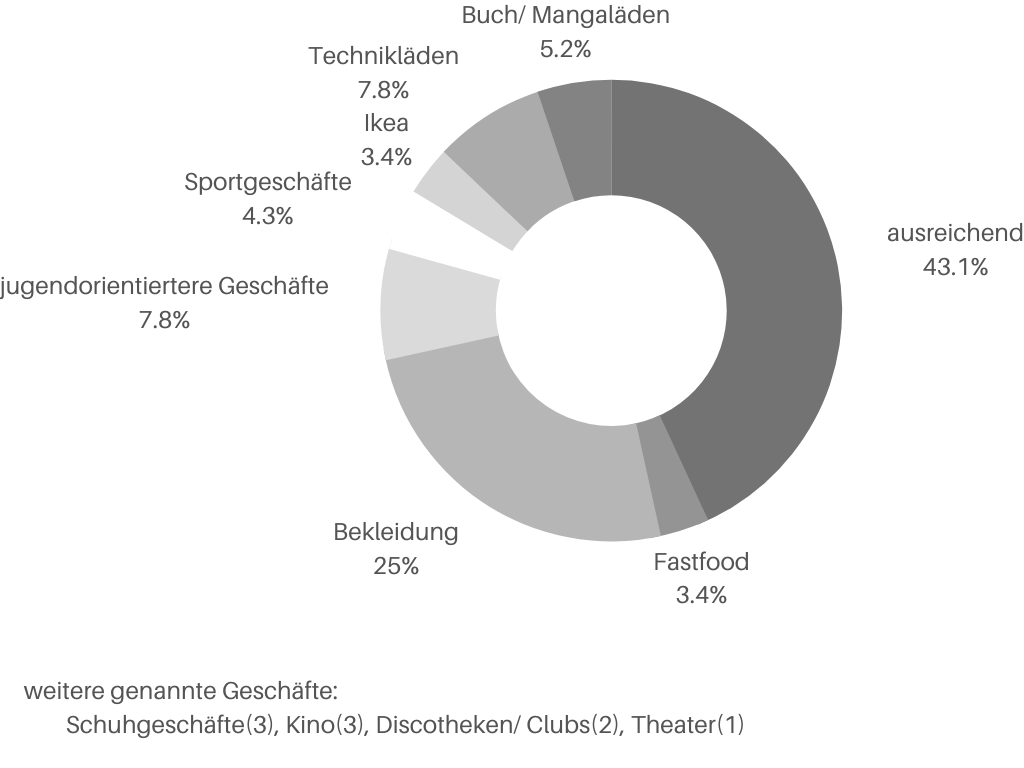
\includegraphics[width=15cm]{media/schuelerumfrage/5.png}
    \end{center}
\end{figure}
\iffalse
Ja: 50

Nein, es fehlt...: Fastfood(4), Bekleidung(29), Schuhgeschäfte(3), Sportgeschäfte(5), Kino(3), Theater(1), Discotheken/ Clubs(2), Technikläden(9), Buch/ Mangaläden(6), Ikea(4), jugendorientierte Geschäfte(9)\\\\
\fi
\newpage\noindent Weichen Sie und ihre Familie beim Einkaufen aufgrund des Angebots auf andere Städte in der Umgebung aus? (6)\\
\iffalse
Nein: 46

Ja: 101: Coburg(46), Suhl(74), Meiningen(3), Erfurt(37), Hildburghausen(12), Zella-Mehlis(10), Bamberg(1)\\\\
\fi

\begin{figure}[H]
    \begin{center}
        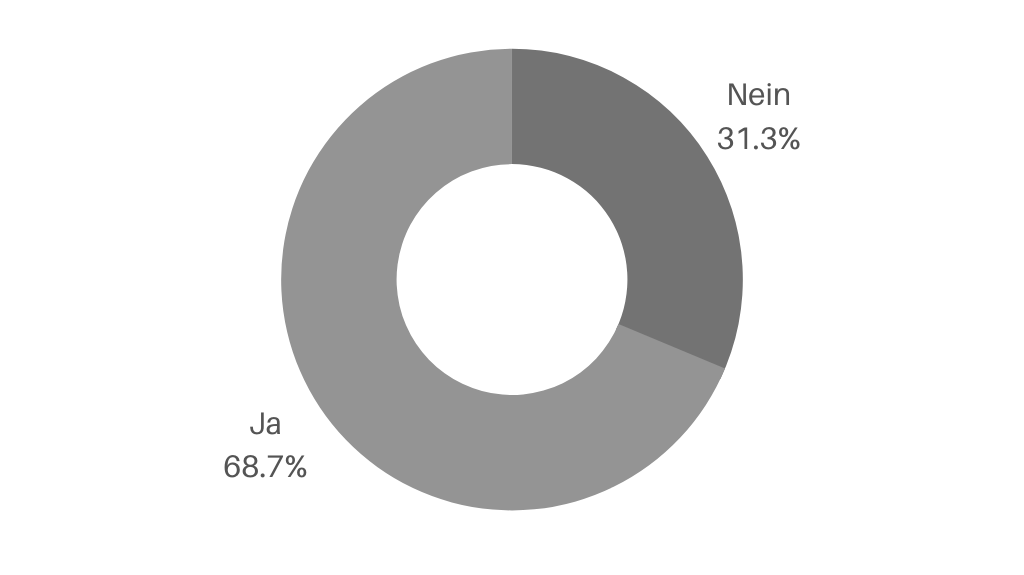
\includegraphics[width=12cm]{media/schuelerumfrage/6.1.png}
    \end{center}
\end{figure}

\begin{figure}[H]
    \begin{center}
        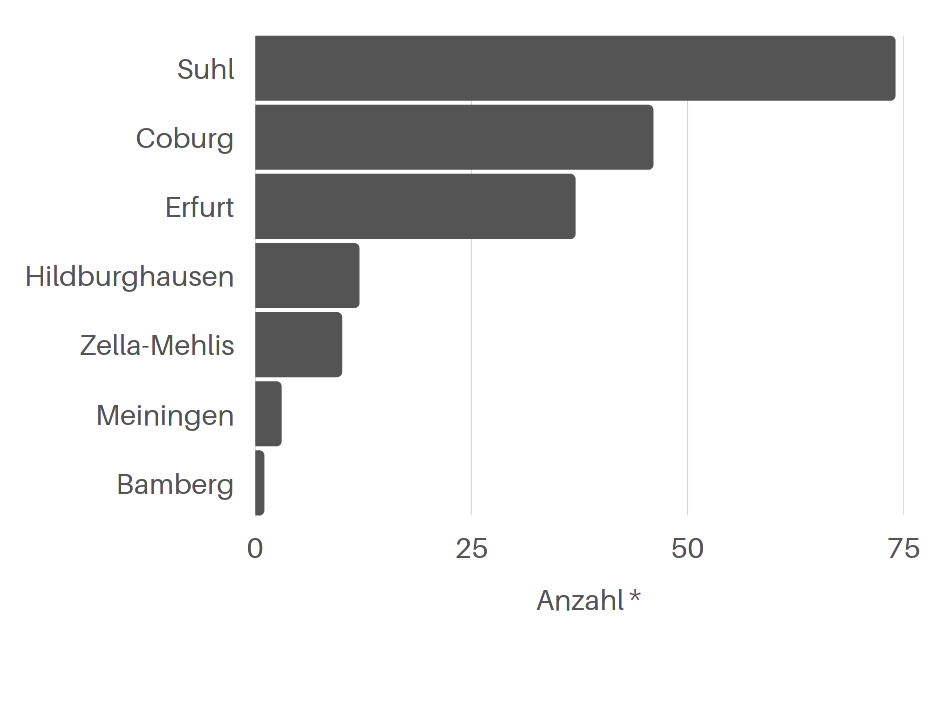
\includegraphics[width=12cm]{media/schuelerumfrage/6.2.png}
    \end{center}
\end{figure}

\newpage\noindent Welche Produkte/ Änderungen im Verkaufsprozess wünschen Sie sich für den Onlinehandel? (7)\\\\

\begin{figure}[H]
    \begin{center}
        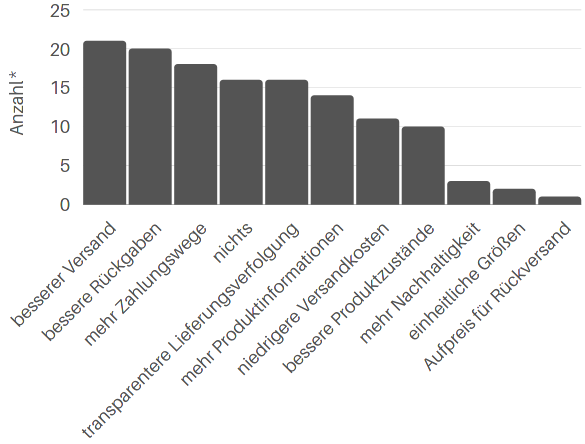
\includegraphics[width=15cm]{media/schuelerumfrage/7.png} 
    \end{center}
\end{figure}
\iffalse
mehr Zahlungswege(9)(Paysafe-Card(3), Paypal(6), Kauf auf Rechnung(3)), mehr Sicherheit(6), besserer Versand(11), transparente Lieferungsverfolgung(8), mehr Produktinformationen(7), einheitliche Größen(1), bessere Rückgaben(10), Nachhaltigkeit(3), bessere Produktzustände(5), niedrigere Versandkosten(5), teuereren Rückversand(1), keine(8)\\\\
\fi
\noindent Welche Produkte/ Änderungen im Verkaufsprozess wünschen Sie sich für den lokalen Handel? (8)\\
\begin{figure}[H]
    \begin{center}
        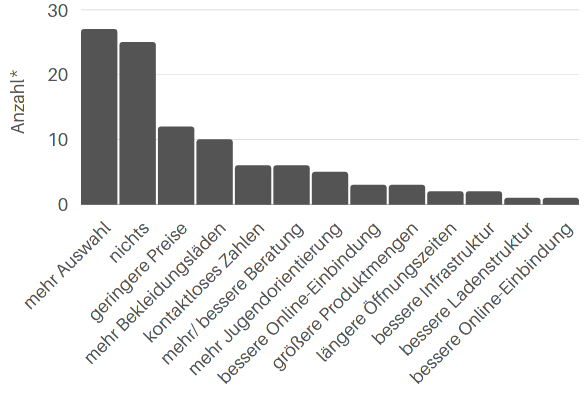
\includegraphics[width=15cm]{media/schuelerumfrage/8.png}
    \end{center} 
\end{figure}
\iffalse
mehr Auswahl(21), mehr/bessere Beratung(5), mehr kulturelles(1), mehr Bekleidung(7), geringere Preise(8), bessere Online-Einbindung(2), größere Produktmengen(2), kontaktloses Zahlen(5), mehr Jugendorientierung(3), längere Öffnungszeiten(2), bessere Infrastruktur(2), bessere Ladenstruktur(1), nichts(19)\\\\
\fi
\newpage\noindent Welche Stärken sehen Sie bzgl. des stationären Einzelhandels im ländlichen Bereich? (9)\\
\begin{figure}[H]
    \begin{center}
        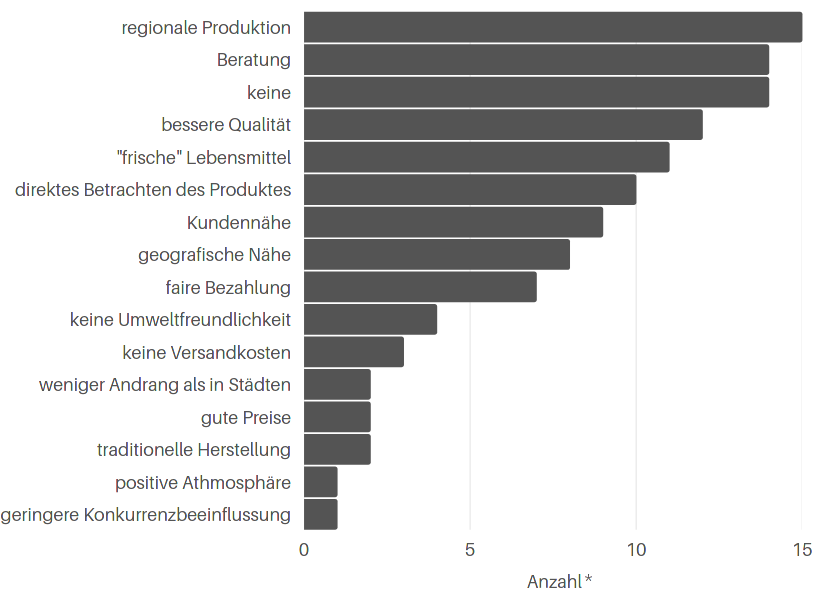
\includegraphics[width=15cm]{media/schuelerumfrage/9.png}
    \end{center}
\end{figure}
\iffalse
Regionale Produktion(13), Umweltfreundlichkeit(3), tradiotionelle Verarbeitung(2), bessere Qualität(9), "frische" Lebensmittel(10), faire Bezahlung(3), geringerer Konkurrenzeinfluss(1), Beratung/ Kundennähe(12/7), gute Preise(2), geografische Nähe(6), Sicherung von Arbeitsplätzen(1), Unterstützung nachgelagerter Strukturen(6), keine Versandkosten(2), weniger Menschen als in Städten(2), positive Athmosphäre(1), direkte Einschätzung des Produktes(8)\\

keine(17)\\\\
\fi
\noindent Kaufen Sie und ihre Familie Gebrauchsgegenstände (mehrfach verwendbare, z. B. Autos, Fernseher usw.) größtenteils neu oder gebraucht? (10)\\

\begin{figure}[H]
    \begin{center}
        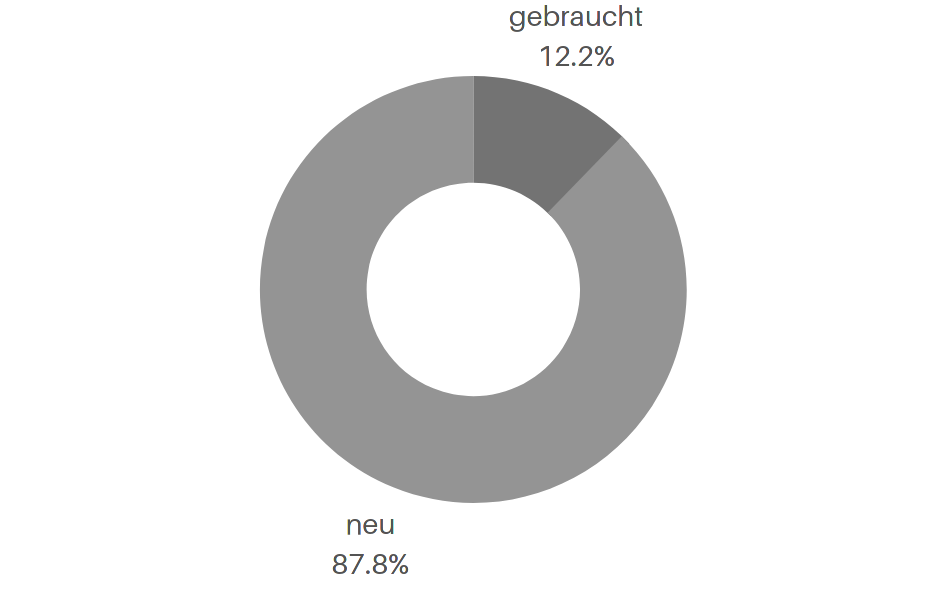
\includegraphics[width=12cm]{media/schuelerumfrage/10.png}
    \end{center}
\end{figure}
\iffalse
neu: 129

gebraucht: 18\\\\
\fi
\newpage\noindent Was ist für Sie relevanter? Der Onlinehandel oder der stationäre Einzelhandel? (11)\\

\begin{figure}[H]
    \begin{center}
        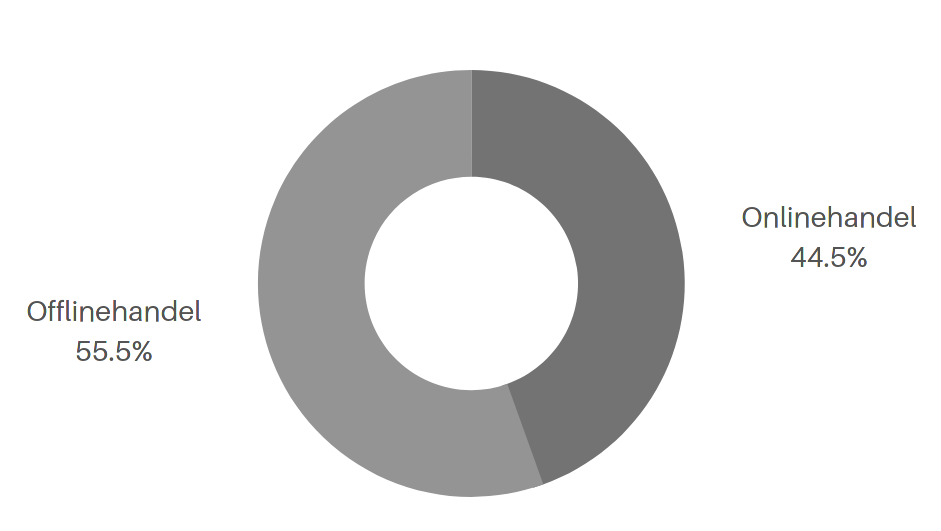
\includegraphics[width=12cm]{media/schuelerumfrage/11.png}
    \end{center}
\end{figure}
\iffalse
Onlinehandel: 61 

Offlinehandel: 76\\\\
\fi
\newpage\noindent Welche Probleme/ Komplikationen sehen sie beim Kauf von Artikeln Online? (12)
\begin{figure}[H]
    \begin{center}
        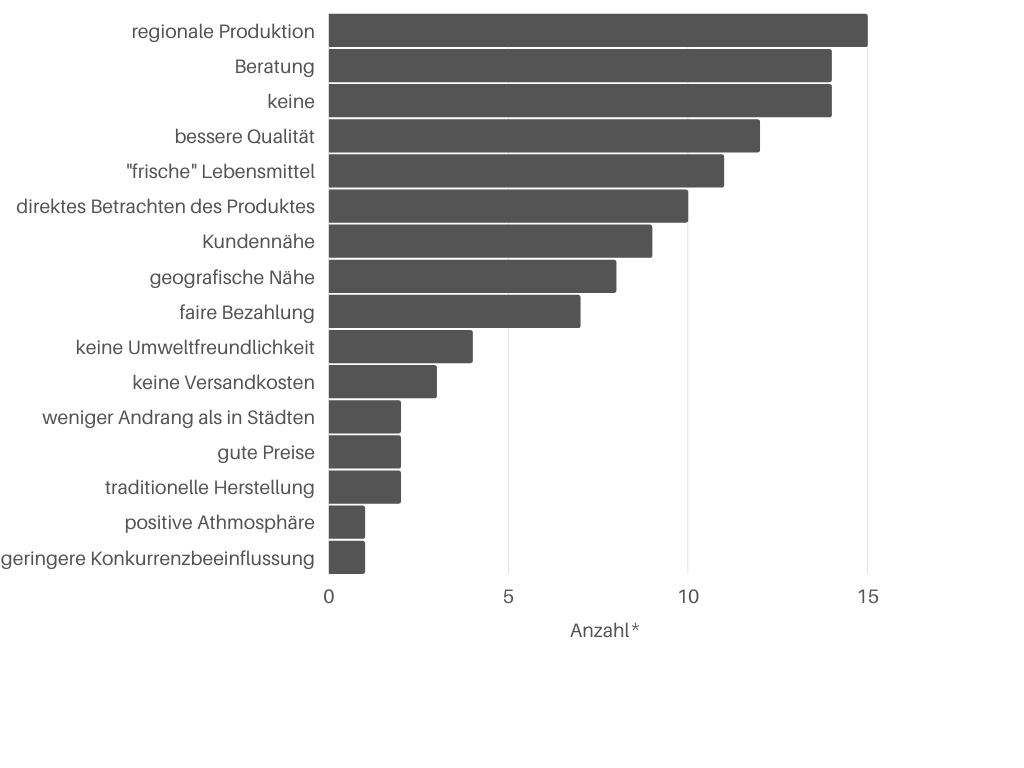
\includegraphics[width=17cm]{media/schuelerumfrage/12.png}
    \end{center}
\end{figure}
\iffalse
keine(10), Betrug(37), Rückgabeprobleme(11), schlechter Produktzustand/ Qualität(34), ungenügende/falsche Produktinformationen(22), Mail/ Post-Spam(2), Versandprobleme(35), Umweltproblematik(5), Größe von Bekleidung(12), Schädigung des Einzelhandels(1), keine Beratung(3)\\\\
\fi
\noindent Wie schätzen sie ihre Preissensibilität ein? (13)\\
 
\begin{figure}[H]
    \begin{center}
        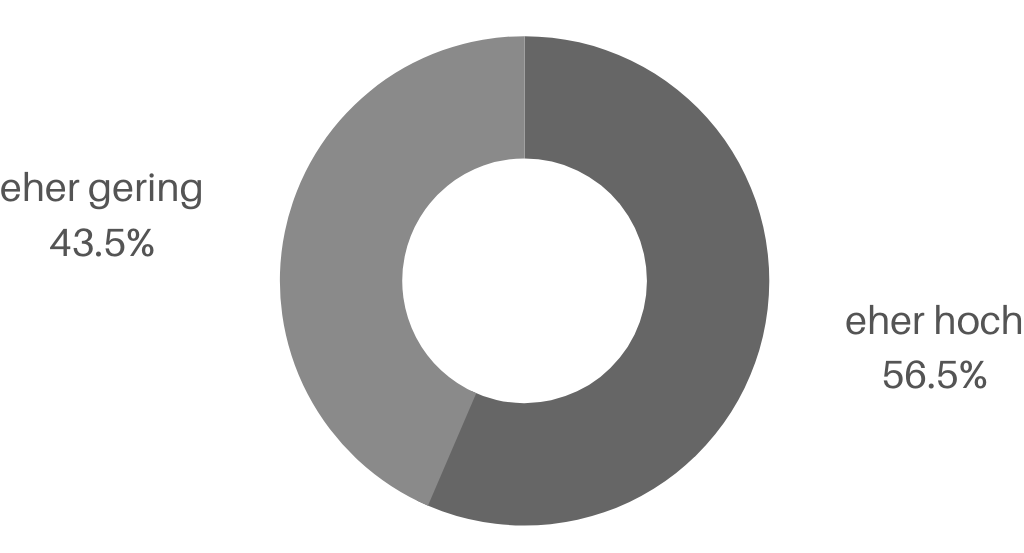
\includegraphics[width=9cm]{media/schuelerumfrage/13.png}
    \end{center}
\end{figure} 
\iffalse
Eher hoch: 83

Eher gering: 64\\\\
\fi
\newpage\noindent Haben sich ihre Kaufgewohnheiten während der Corona-Zeit geändert? (14)\vfill

\begin{figure}[H]
    \begin{center}
        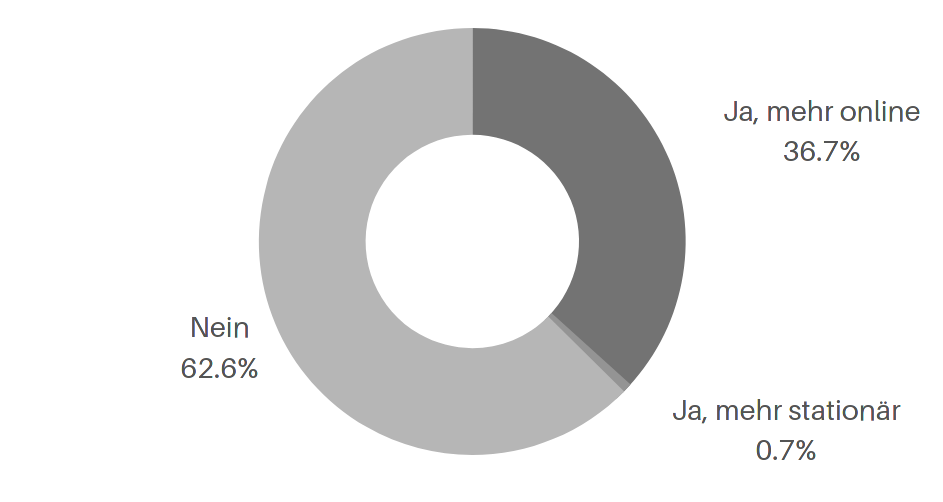
\includegraphics[width=12cm]{media/schuelerumfrage/14.png}
    \end{center}
\end{figure}
\iffalse
Nein: 92

Ja, mehr stationär: 0

Ja, mehr online: 55\\\\\\
\fi
\vfill\vfill
\noindent Wann haben Sie das erste mal etwas online gekauft? (15)\vfill

\begin{figure}[H]
    \begin{center}
        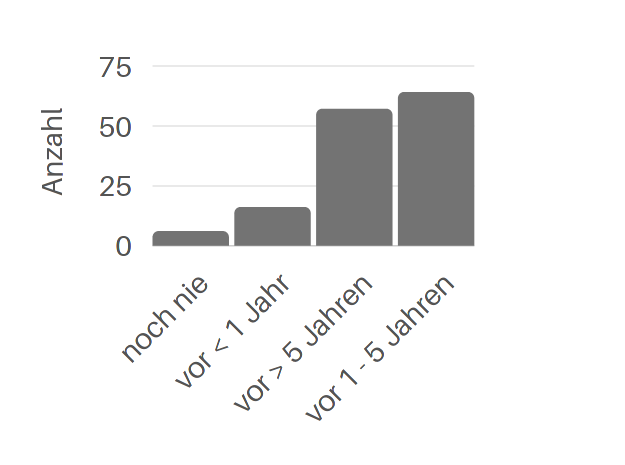
\includegraphics[width=8cm]{media/schuelerumfrage/15.png}
    \end{center}
\end{figure} 
\vfill
\iffalse
Noch nie: 6

Vor 5 oder mehr Jahren: 64

Vor 1-5 Jahren: 57

Vor 1 Jahr oder später: 16
\fi












